% lehr-sphere.tex

\newpage
\section{Flow of detonable mixture over a sphere}
\index{chemical reaction!example of use}
\index{gas model!thermally perfect!example of use}
%
Interesting things can happen when the chemical-reaction time scales
are of the same order as the flow time scales. 
This example simulates the flow of a stoichiometric mixture of hydrogen and air over
the spherical nose of a projectile as used by Lehr in some ballistic range experiments
\cite{lehr_1972}.
For a range of Mach numbers, the combustion of the hydrogen is unsteady so it provides
an interesting test of the interaction of the gas dynamics and chemical kinetics modules
of the code.
Figure\,\ref{lehr-expt-M479-fig} shows the periodic structure caused by the unsteady combustion 
of the gas mixture over the projectile.

\begin{figure}[htbp]
\begin{center}
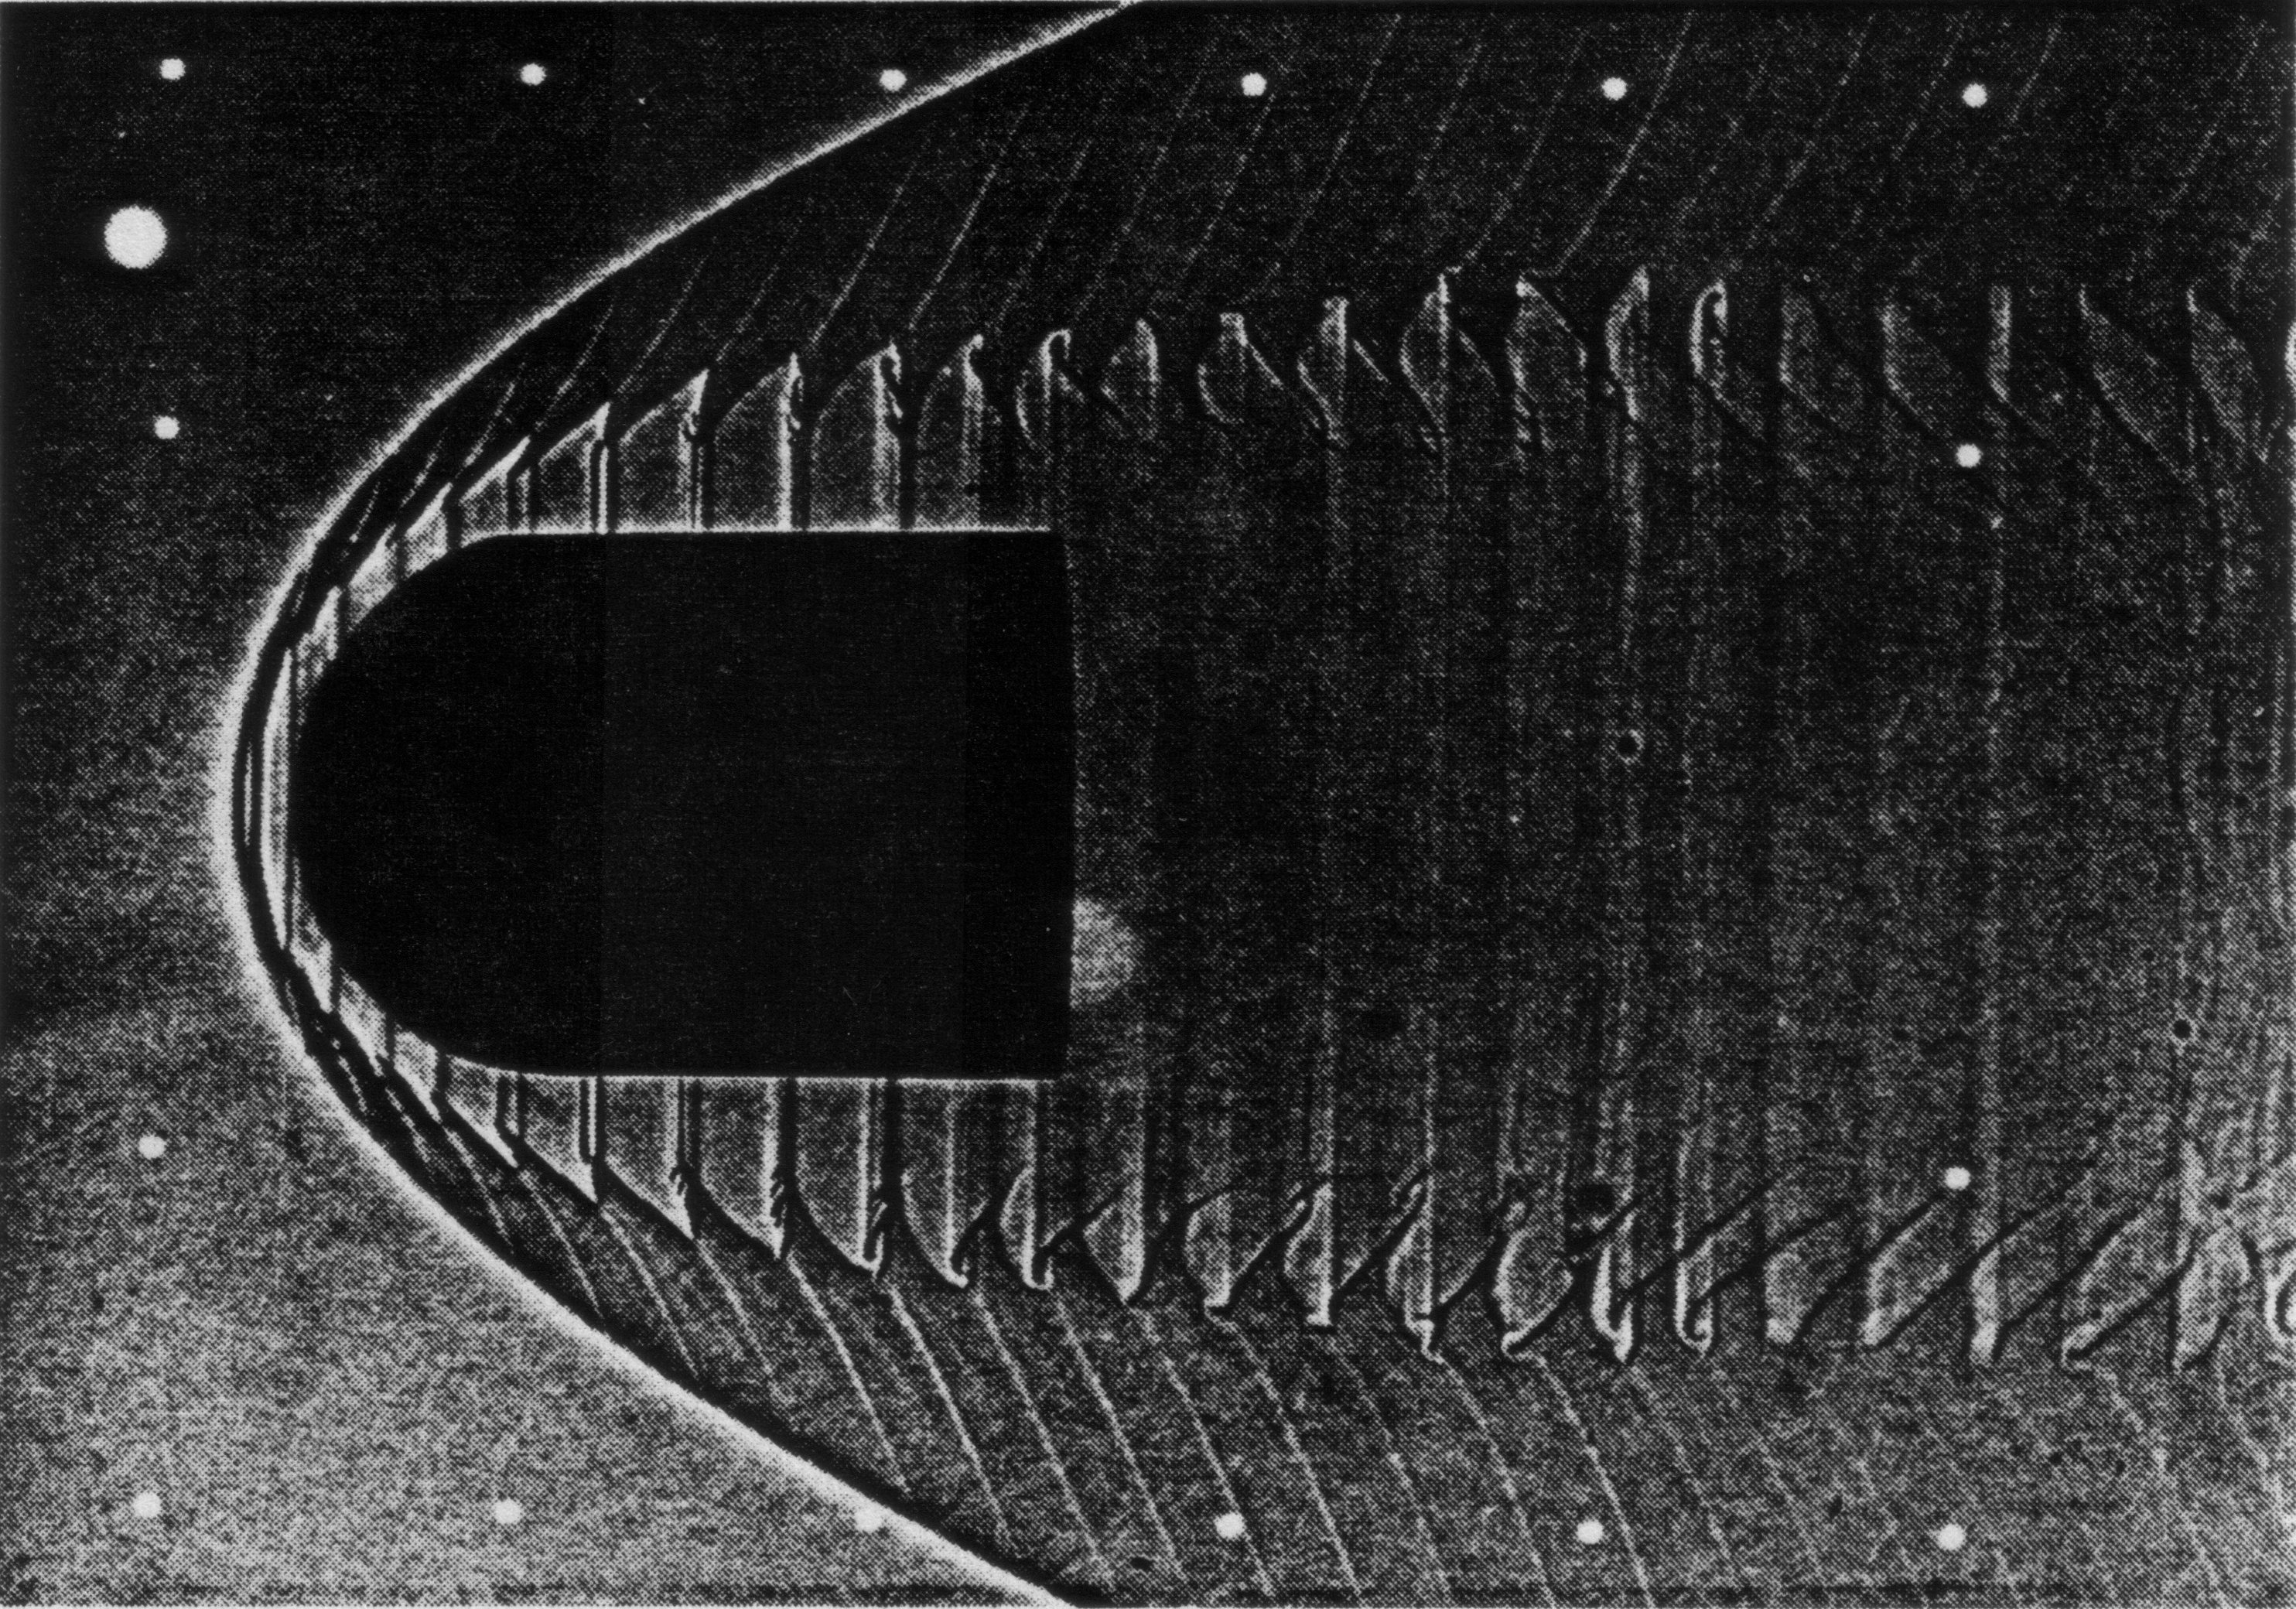
\includegraphics[width=10cm]{../2D/lehr-479/lehr-M4p79-scanned-image-from-wilson-thesis.jpg}
\end{center}
\caption{Shadowgraph of the unsteady flow of reacting hydrogen and air over a ballistic-range
  projectile at a Mach number of 4.79.  This particular image has been scanned from Greg Wilson's
  PhD thesis \cite{wilson_1991}.}
\label{lehr-expt-M479-fig}
\end{figure}

\medskip
The free-stream condition is $p_{\infty} = 320$\,mm\,Hg, $T_{\infty} = 292$\,K,
$u_{\infty} = 1.931$\,km/s, corresponding to a Mach number of 4.79 in a stoichiometric mixture
of hydrogen and air (nitrogen + oxygen only).
The small calculation to get actual mass fraction of each species is done as part of the user input script.
For this flight condition, Lehr observed a frequency of oscillation of 0.72\,MHz. 

\medskip
Because this example is just a demonstration of the code capability and not a validation
and because the case takes a day or two to run on 4 processors of geyser,
we settle for the use of a reduced chemical reaction scheme in which nitrogen is assumed to be
a non-reacting diluent gas.
This is done near the top of the the reaction scheme file \ref{lehr-reaction-file} 
by selecting \texttt{INERT\_N2} as the model.

\begin{figure}[htbp]
\begin{center}
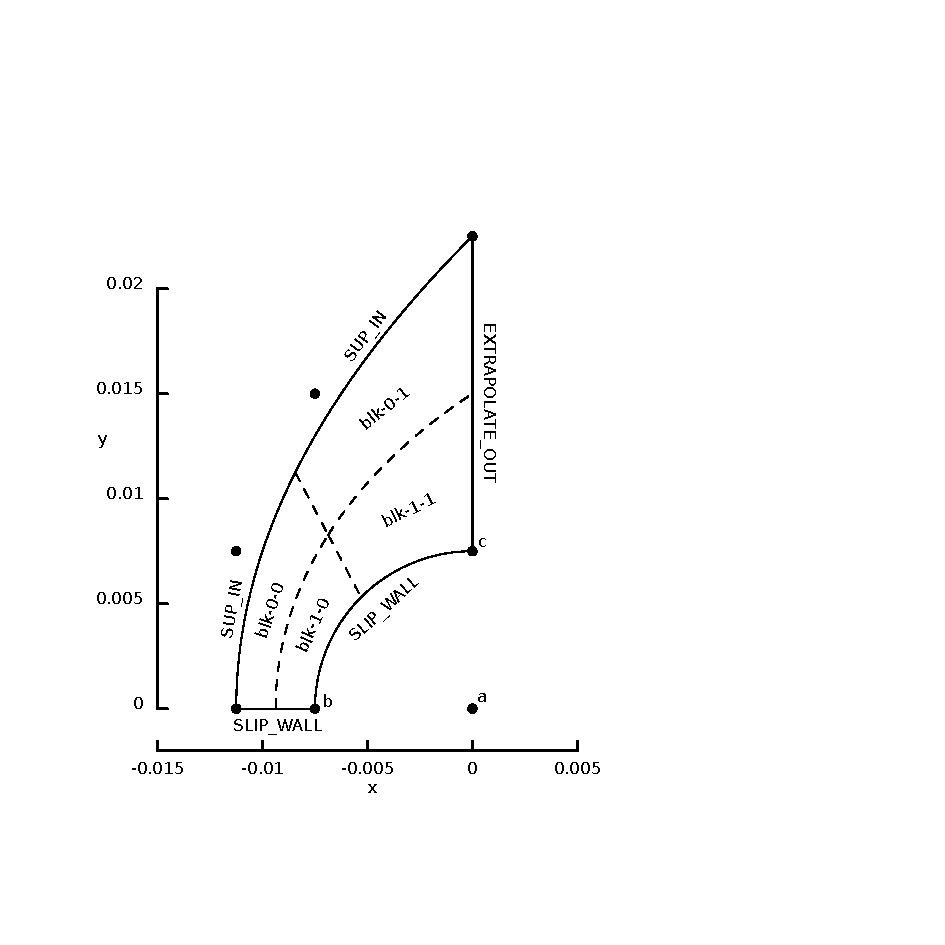
\includegraphics[width=10cm,viewport=43 73 288 344,clip=true]{../2D/lehr-479/lehr-layout.pdf}
\end{center}
\caption{Schematic diagram of the geometry for a sphere wrapped by a SuperBlock2D grid.
   Although $2 \times 2$ blocks are shown here, we are typically impatient and 
   use $4 \times 6$ blocks as shown in the input scripts.}
\label{lehr-geometry-fig}
\end{figure}

\medskip
If we start very reasonably, with a low-resolution grid and do the calculation fairly in short order,
we get something like the left image in Figure\,\ref{lehr-T-field-fig}.
The solution is all very steady, well behaved, and quite wrong.
The reaction front has merged into the shock and the whole shock layer has inflated to a stand-off distance
significantly larger than that observed in the experiment.
Just increasing the grid resolution (by a factor of 10 in each direction) provided a solution as shown in the right
side of Figure\,\ref{lehr-T-field-fig}.
Here, the reaction front is clearly separated from the incident shock, and it is not smooth.
Although it is not clear from this particular image, there is a periodic large scale disturbance 
to the reaction front, and a slightly smaller disturbance to the shock front.

\begin{figure}[htbp]
\begin{center}
\mbox{
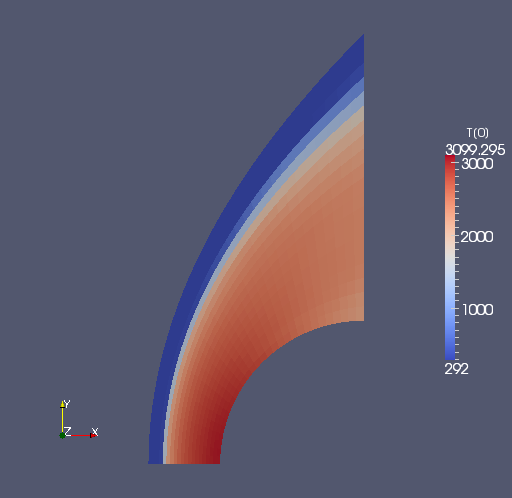
\includegraphics[width=0.45\textwidth]{../2D/lehr-479/lehr-479-T-field-t0019-20x30.png}
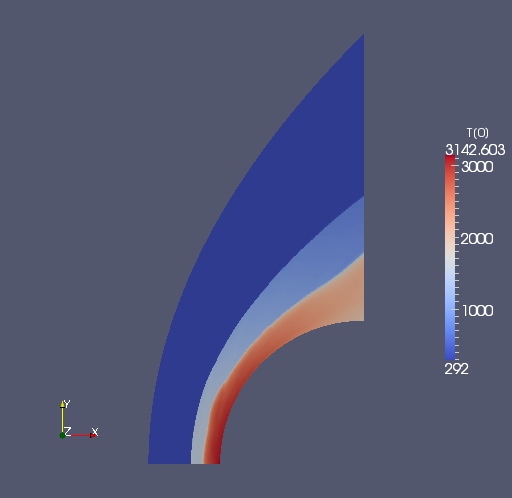
\includegraphics[width=0.45\textwidth]{../2D/lehr-479/lehr-479-T-field-t0019-200x300.png}
}
\end{center}
\caption{Temperature field at t=190\,$\mu$s for 20$\times$30 cells (left) and 200$\times$300 cells (right).}
\label{lehr-T-field-fig}
\end{figure}

\medskip
Figure \ref{lehr-density-field-fig} shows the density field for a few frames 
of the second-stage simulation (\texttt{lehr1.py}) over roughly one period of the large-scale oscillation.
Although the periodic nature of the flow is captured, the detailed behaviour of the reaction front 
is quite sensitive to grid resolution and the details of the reaction mechanism.
The frequency of the large scale oscillation in this simulation is a long way short of the 0.72\,MHz 
observed by Lehr.
It is left as an exercise for the reader to try the more complete reaction schemes to see if the frequency 
of the flow oscillation can be better approximated.

\begin{figure}[htbp]
\begin{center}
\mbox{
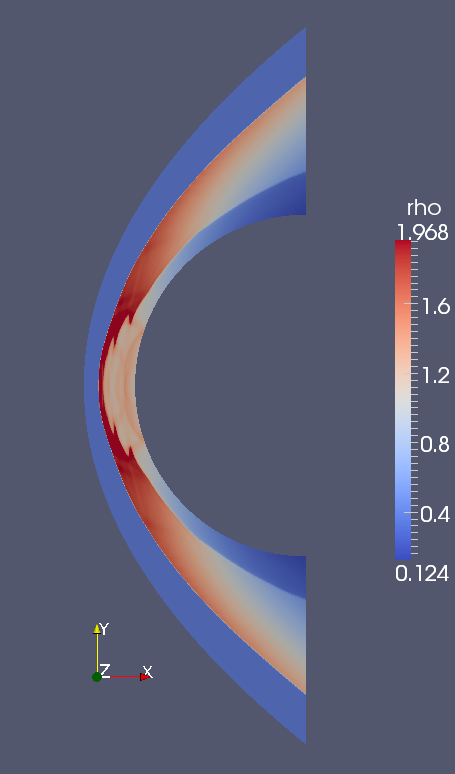
\includegraphics[width=0.25\textwidth]{../2D/lehr-479/lehr1-density-field-200x300-frame-11.png}
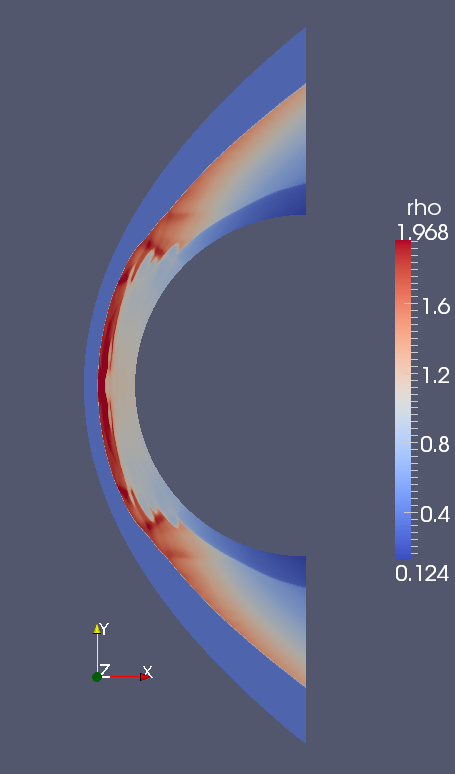
\includegraphics[width=0.25\textwidth]{../2D/lehr-479/lehr1-density-field-200x300-frame-14.png}
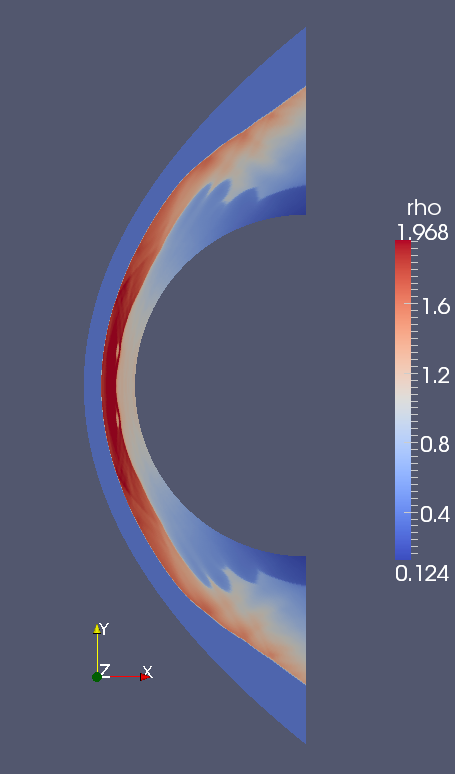
\includegraphics[width=0.25\textwidth]{../2D/lehr-479/lehr1-density-field-200x300-frame-17.png}
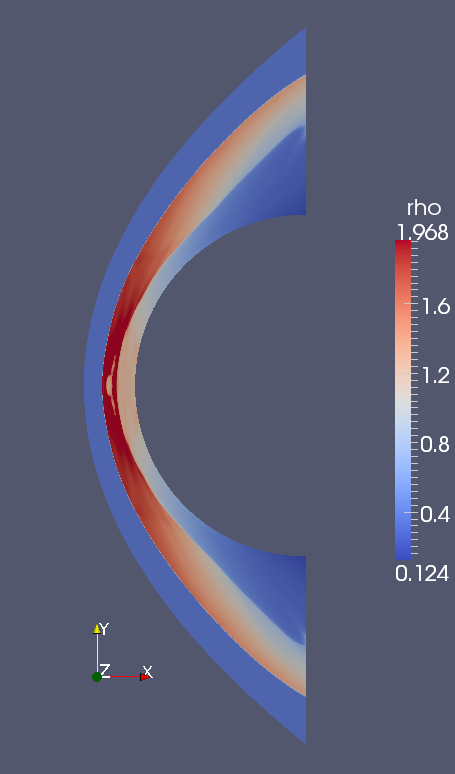
\includegraphics[width=0.25\textwidth]{../2D/lehr-479/lehr1-density-field-200x300-frame-20.png}
}
\end{center}
\caption{Density field at t=11, 14, 17, 20\,$\mu$s in the \texttt{lehr1} second-stage simulation.}
\label{lehr-density-field-fig}
\end{figure}


\subsection{Input script (.py)}
\topbar
\lstinputlisting[language={}]{../2D/lehr-479/lehr.py}
\bottombar

\medskip\noindent
The second input script continues the simulation on a grid where the inflow boundary 
has been moved in toward the bow shock.
This makes better use of the computational resources as more cells are now within the shock layer.
\index{ExistingSolution!example of use}

\noindent
\topbar
\lstinputlisting[language={}]{../2D/lehr-479/lehr1.py}
\bottombar

\newpage
\subsection{Reaction scheme file (.lua)}\index{chemical reaction!reaction scheme file!H2-air combustion}
\label{lehr-reaction-file}
\topbar
\lstinputlisting[language={}]{../2D/lehr-479/Evans_Schexnayder.lua}
\bottombar

\medskip
\subsection{Notes}
\begin{itemize}
\item None
\end{itemize}
